\section{Introduction}
\label{intro}

With success of unsupervised representation learning in NLP, pretrained language 
models, such as BERT and RoBERTa, have achieved a superhuman 
performance across many popular reasoning classification tasks, like NLI~\cite{} and FEVER~\cite{}. 
%Each instance in NLI dataset consists of a premise-hypothesis pair that belongs to one
%out of three possible categories (entailment, contradiction, or neutral) based on the relationship
%between the premise and the hypothesis. 
%\figref{fig:example}  shows an example of
%a NLI premise and hypothesis. 
%\YZ{
The NLI dataset consists of premise-hypothesis pairs. 
As shown in \figref{fig:example}, the relationship between premise and hypothesis in one pair
is one out of three   
possible categories (entailment, contradiction, or neutral).
%}
As a reasoning classification problem,
FEVER, the task of fact verification, 
%involves assessing
%claim validity in the context of evidence, which
%can support, refute or contain not enough
%information. 
%\YZ{
assesses whether the evidence supports the claim, refutes the claim, 
or fails to determine the validity of the claim due to not enough information. 
%}
\figref{fig:example} shows 
a FEVER claim and its evidence.

\begin{figure}[th!]
	\centering
	\includegraphics[width=0.4\columnwidth]{figures/noise_example.eps}
	\caption{SNLI and FEVER examples}
	\label{fig:example}
\end{figure}

Benefit from deeper neutral 
network and larger learning materials, these models should have a better comprehension 
and reasoning ability. Yet these deep models struggle when taken out of these dataset environments and evaluated
on adversarial data or problems out of domain~\cite{},
%\YZ{What do you mean by these data? You use spurious cues in abstract and use spurious features in intro, are they same? What is spurious features or cues?}
%which indicates that those datasets overestimate the true capabilities of current models due to spurious features 
%existing in datasets.
%\YZ{
which indicates that the true capabilities of existing models are overestimated due to superficial patterns in current datasets.
%}

Superficial pattern analysis is hot in recent research. Since 
lots of work~\cite{} 
have shown that many models can even 
get good performance without observing the stem of  multiple choice questions.
There are mainly two types of superficial patterns which have been observed in many datasets~\cite{}: 
%lexicalized and unlexicalized~\cite{}.
%Lexicalized feature Unlexicalized features 
shallow n-gram distribution patterns which mainly contains the indicator of n-gram tokens and cross-ngram tokens.
and overlap features involving  lexical overlap heuristic, 
subsequence heuristic and constituent heuristic~\cite{} 
assuming that a premise entails all
hypotheses constructed from words
in the premise. In addition, a more 
intuitive phenomenon is that even without premise in NLI tasks or evidence in FEVER, 
the models can still have a pretty good performance. These spurious features can 
impact the generalization and robustness of models~\cite{}.

%we further investigate
%the lexicalized irregularities, what we refer as spurious tokens which can mostly 
%change the result of instances. 
Existing techniques to improve the quality of the datasets 
include data filtering and data augmentation.  
The data filtering model~\cite{bras2020adversarial} 
produces a reduced dataset with fewer spurious features through iteratively 
training on complex neural network models. 
%\YZ{You mean that the data filtering models produces a new dataset by complex neural based model?}
However, they also leave out many
 importance learning materials (even less than 10\% are retained). 
The data augmentation, collecting more data manually,
is too expensive. Thus, some work~\cite{} automatically generate 
more training data in which neutralizes some 
superficial patterns by designed logic rules. 
But these generation logical can also become new kinds of spurious features~\cite{}.

In this paper, we propose a new data augmentation method
to enhance the robustness,
called noise data augmentation.
%by disregarding the simple spurious features 
%and turning to focus more on other more meaningful and perhaps more sophisticated features. . 
The ``noise'' here may be different from the definition of noise in computer vision~\cite{}. 
%In fact, the ``noise'' data is not wrong or counterfactual with the corresponding label. 
%\YZ{
In fact, the ``noise'' data are not the instances with wrong or counterfactual labels.
%}
For the SNLI example in~\figref{fig:example}, we will never choose ``Entailment'' 
for the original instance as a new noise sample because this is wrong.
We generate ``noise'' instances for datasets which doesn't conform to grammar 
or inferential format with a new label ``Noise'',
and combine with original instances to form a new augmented dataset and we call it noise dataset. 
%\YZ{It is not clear. noise instances, original instances? You mean you add noise instances into dataset?}
The external label ``Noise'' corresponds to a new relation between the \textit{premise} and \textit{hypothesis}
or between \textit{claim} and \textit{evidence} 
which means this instance is a broken one like the instance doesn't 
have a \textit{premise} or \textit{evidence}. 
%\YZ{Give an example of instance with label Noise ?}
Our target for generating data is to optimize %\YZ{maybe another word is better. How about ``optimize''?}                       
the model, which can 
increase the difficulty of training so that the model cannot be easily
fitted with shallow spurious features and focuses on more complex features.
  
According to unbalanced token distribution, overlap 
and hypothesis-only (or claim-only) superficial patterns we 
mentioned above, we generate noise data from three aspects. 
First, we balance the frequency of tokens in original dataset with new instances.
The generated ones are only a set of words which don't grammatical. 
Models can not easily make decisions only for the appearance of words. 
Second, we random replace some words in \textit{hypothesis} (or \textit{claim}) 
with words in \textit{premise} (or \textit{evidence}) 
to simulate tokens overlap in an instance. For example, we take ``playing rope are bad nobody with church 
you when the a.'' as the new premise of a noise instance which shares ``playing'', ``rope'' and ``nobody'' 
with \textit{hypothesis} ``Nobody is playing jump rope.''
Third, we add hypothesis-only (or claim-only) noise intuitively. 
% These three methods can give more training data with an extra label ``Noise". 
%We try different types and proportions of noise data augmentation.
The models retrained on our new augmentation data have a consistent performance on 
original test dataset datasets and outperform the models
trained on original on challenging adversarial datasets~\secref{sec:dataset}. 
%original dataset and stress test \YZ{original test set and stress test set? Do you need explain what stress test is?}, which 
%shows the retrained models are more robust.with the model 
%trained on original 
%We generate premise-hypothesis pairs with label "Noise" automatic 
%by random choosing a premise and generate a hypothesis with random 
%choose some some words from the whole corpus beyond grammar. 
%We also control the sentence length with average length in original dataset.

%Our contribution of this paper can be summarized in
%two-fold:




%1) We can only consider the frequency, which means the words frequency in 
%our generation part will be equal to the max number in each original labeled part.

%not influenced by "Noise", reasons:1. have no distribution noise. 2.not a sentence, but bert is based on sentence, fasttext may be influence.


%2) We can just delete the premise

%3) We can  change the ending order 


